\subsection{DECOMPOSABLE LINEAR LIE ALGEBRAS}

DEFINITION 1. Let g be a Lie subalgebra of \(\mathfrak{gl}(V)\) . Then g is said to be decomposable if g contains the semi-simple and nilpotent components of each of its elements (Algebra, Chap. VII, §5, no. 8).

Examples. 1) Let \(V'\) and \(V''\) be vector subspaces of V such that \(V'' \supset V'\) . The set of \(x \in \mathfrak{gl}(V)\) such that \(x(V'') \subset V'\) is a decomposable Lie subalgebra of \(\mathfrak{gl}(V)\) ; indeed, for all \(x \in \mathfrak{gl}(V)\) , the semi-simple and nilpotent components of x are of the form \(P(x)\) and \(Q(x)\) , where P and Q are polynomials without constant term.

\begin{enumerate}
\def\labelenumi{\arabic{enumi})}
\setcounter{enumi}{1}
\item
  Assume that V has an algebra structure. The set of derivations of V is a decomposable Lie subalgebra of \(\mathfrak{gl}(V)\) (§1, no. 1, Prop. 4 (ii)).
\item
  \emph{More generally, it can be shown that the Lie algebra of any algebraic subgroup of \(\mathbf{GL}(\mathrm{V})\) is decomposable.}
\end{enumerate}

PROPOSITION 1. Let \(\mathfrak{g}\) be a decomposable Lie subalgebra of \(\mathfrak{gl}(\mathrm{V})\) , \(x \in \mathfrak{g}\) , \(s\) and \(n\) the semi-simple and nilpotent components of \(x\) .

\begin{enumerate}
\def\labelenumi{(\roman{enumi})}
\item
  The semi-simple and nilpotent components of \(\operatorname{ad}_{\mathfrak{g}}x\) are \(\operatorname{ad}_{\mathfrak{g}}s\) and \(\operatorname{ad}_{\mathfrak{g}}n\) , respectively.
\item
  \(x\) is regular in \(\mathfrak{g}\) if and only if \(s\) is.
\item
  If \(\mathfrak{g}'\) is a subalgebra of \(\mathfrak{gl}(\mathrm{V})\) containing \(\mathfrak{g}\) , every elementary automorphism of \(\mathfrak{g}\) extends to an elementary automorphism of \(\mathfrak{g}'\) .
\end{enumerate}

Put \(\mathfrak{a} = \mathfrak{gl}(V)\) . By Chap. I, §5, no. 4, Lemma 2, the semi-simple and nilpotent components of \(\mathrm{ad}_{\mathfrak{a}}x\) are \(\mathrm{ad}_{\mathfrak{a}}s\) and \(\mathrm{ad}_{\mathfrak{a}}n\) ; assertion (i) follows from this. We deduce that the characteristic polynomials of \(\mathrm{ad}_{\mathfrak{g}}x\) and \(\mathrm{ad}_{\mathfrak{g}}s\) are the same; hence (ii). If \(\mathrm{ad}_{\mathfrak{g}}x\) is nilpotent, \(\mathrm{ad}_{\mathfrak{g}}x = \mathrm{ad}_{\mathfrak{g}}n\) , so \(\mathrm{ad}_{\mathfrak{g}'}n\) extends \(\mathrm{ad}_{\mathfrak{g}}x\) , and \(n\) is a nilpotent element of \(\mathfrak{g}'\) , hence (iii).

Let \(\mathfrak{g}\) be a Lie subalgebra of \(\mathfrak{gl}(\mathrm{V})\) . We know (Chap. I, §6, no. 5, Th. 4) that the following conditions are equivalent:

\begin{enumerate}
\def\labelenumi{(\roman{enumi})}
\item
  the identity representation of \(\mathfrak{g}\) is semi-simple;
\item
  \(\mathfrak{g}\) is reductive and every element of the centre of \(\mathfrak{g}\) is a semi-simple endomorphism.
\end{enumerate}

These conditions are actually equivalent to the following:

\begin{enumerate}
\def\labelenumi{(\roman{enumi})}
\setcounter{enumi}{2}
\tightlist
\item
  \(\mathfrak{g}\) is a reductive subalgebra in \(\mathfrak{gl}(\mathrm{V})\) .
\end{enumerate}

Indeed, (i) \(\Longrightarrow\) (iii) by Chap. I, §6, no. 5, Cor. 3 of Th. 4, and (iii) \(\Longrightarrow\) (i) by Chap. I, §6, no. 6, Cor. 1 of Prop. 7. We are going to show that if \(\mathfrak{g}\) satisfies these conditions, \(\mathfrak{g}\) is decomposable. More generally:

PROPOSITION 2. Let g be a Lie subalgebra of \(\mathfrak{gl}(V)\) reductive in \(\mathfrak{gl}(V)\) , E a finite dimensional vector space and \(\pi : g \to \mathfrak{gl}(E)\) a semi-simple linear representation of g on E. Then:

\begin{enumerate}
\def\labelenumi{(\roman{enumi})}
\item
  \(\mathfrak{g}\) and \(\pi (\mathfrak{g})\) are decomposable.
\item
  The semi-simple (resp. nilpotent) elements of \(\pi(\mathfrak{g})\) are the images under \(\pi\) of the semi-simple (resp. nilpotent) elements of \(\mathfrak{g}\) .
\item
  If \(\mathfrak{h}\) is a decomposable subalgebra of \(\mathfrak{gl}(\mathrm{V})\) contained in \(\mathfrak{g}\) , \(\pi(\mathfrak{h})\) is a decomposable subalgebra of \(\mathfrak{gl}(\mathrm{E})\) .
\item
  If \(\mathfrak{h}'\) is a decomposable subalgebra of \(\mathfrak{gl}(\mathrm{E})\) , \(\pi^{-1}(\mathfrak{h}')\) is a decomposable subalgebra of \(\mathfrak{gl}(\mathrm{V})\) .
\end{enumerate}

Let \(\mathfrak{s} = [\mathfrak{g},\mathfrak{g}]\) and let \(\mathfrak{c}\) be the centre of \(\mathfrak{g}\) . Then \(\mathfrak{g} = \mathfrak{s} \times \mathfrak{c}\) , and \(\pi(\mathfrak{g}) = \pi(\mathfrak{s}) \times \pi(\mathfrak{c})\) by Chap. I, §6, no. 4, Cor. of Prop. 5. Let \(y \in \mathfrak{s}, z \in \mathfrak{c}, y_s\) and \(y_n\) the semi-simple and nilpotent components of \(y\) . Then \(y_s, y_n \in \mathfrak{s}\) (Chap. I, §6, no. 3, Prop. 3), \(y_s + z\) is semi-simple (Algebra, Chap. VII, §5, no. 7, Cor. of Prop. 16), and \(y_n\) commutes with \(y_s + z\) . Hence, the semi-simple and nilpotent components of \(y + z\) are \(y_{s} + z\) and \(y_{n}\) . Thus, g is decomposable. Since \(\pi(\mathfrak{g})\) is reductive in \(\mathfrak{gl}(\mathrm{E})\) , the same argument applies to \(\pi(\mathfrak{g})\) and shows that \(\pi(\mathfrak{g})\) is decomposable. Moreover, the nilpotent elements of g (resp. \(\pi(\mathfrak{g})\) ) are the nilpotent elements of s (resp. \(\pi(\mathfrak{s})\) ). Hence the nilpotent elements of \(\pi(\mathfrak{g})\) are the images under \(\pi\) of the nilpotent elements of g (Chap. I, §6, no. 3, Prop. 4). The semi-simple elements of g (resp. \(\pi(\mathfrak{g})\) ) are the sums of the semi-simple elements of s (resp. \(\pi(\mathfrak{s})\) ) and the elements of c (resp. \(\pi(\mathfrak{c})\) ). Thus the semi-simple elements of \(\pi(\mathfrak{g})\) are the images under \(\pi\) of the semi-simple elements of g (Chap. I, loc. cit.). Hence (ii).

Assertions (iii) and (iv) follow immediately from (i) and (ii).

Remarks. 1) The semi-simplicity assumption on \(\pi\) is equivalent to saying that \(\pi(x)\) is semi-simple for all \(x \in \mathfrak{c}\) . Note that this assumption is satisfied when \(\pi\) is obtained from the identity representation \(\mathfrak{g} \to \mathfrak{gl}(V)\) by the successive application of the following operations: tensor product, passage to the dual, to a subrepresentation, to a quotient, to a direct sum.

\pandocbounded{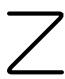
\includegraphics[keepaspectratio]{images/part001_3ab49149.jpg}}

\begin{enumerate}
\def\labelenumi{\arabic{enumi})}
\setcounter{enumi}{1}
\tightlist
\item
  Let \(\mathfrak{g} \subset \mathfrak{gl}(V)\) , \(\mathfrak{g}' \subset \mathfrak{gl}(V')\) be decomposable Lie algebras, \(\varphi\) an isomorphism from \(\mathfrak{g}\) to \(\mathfrak{g}'\) . Note that \(\varphi\) does not necessarily transform semi-simple (resp. nilpotent) elements of \(\mathfrak{g}\) to semi-simple (resp. nilpotent) elements of \(\mathfrak{g}'\) (Exerc. 2). However, this is the case if \(\mathfrak{g}\) is semi-simple (Chap. I, §6, no. 3, Th. 3).
\end{enumerate}

PROPOSITION 3. Let \(\mathfrak{a}\) be a decomposable Lie subalgebra of \(\mathfrak{gl}(\mathrm{V})\) and let \(\mathfrak{b}\) and \(\mathfrak{c}\) be vector subspaces of \(\mathfrak{gl}(\mathrm{V})\) such that \(\mathfrak{b} \subset \mathfrak{c}\) . Let \(\mathfrak{a}'\) be the set of \(x \in \mathfrak{a}\) such that \([x, \mathfrak{c}] \subset \mathfrak{b}\) . Then \(\mathfrak{a}'\) is decomposable.

Put \(\mathfrak{g} = \mathfrak{gl}(\mathrm{V})\) ; the subalgebra \(\mathfrak{h}'\) of \(\mathfrak{gl}(\mathfrak{g})\) consisting of the \(z \in \mathfrak{gl}(\mathfrak{g})\) such that \(z(\mathfrak{c}) \subset \mathfrak{b}\) is decomposable (Example 1). Let \(\pi : \mathfrak{g} \to \mathfrak{gl}(\mathfrak{g})\) be the adjoint representation of \(\mathfrak{g}\) . Prop. 2 (iv), applied to \(\pi\) , shows that \(\pi^{-1}(\mathfrak{h}')\) is decomposable. Hence so is \(\mathfrak{a}' = \mathfrak{a} \cap \pi^{-1}(\mathfrak{h}')\) .

COROLLARY 1. If \(\mathfrak{a}\) is a decomposable Lie subalgebra of \(\mathfrak{gl}(\mathrm{V})\) , and \(\mathfrak{n}\) a Lie subalgebra of \(\mathfrak{a}\) , the normalizer (resp. centralizer) of \(\mathfrak{n}\) in \(\mathfrak{a}\) is decomposable.

This follows from Prop. 3 by taking \(\mathfrak{c} = \mathfrak{n},\mathfrak{b} = \mathfrak{n}\) (resp. \(\mathfrak{c} = \mathfrak{n},\mathfrak{b} = \{0\}\) ).

COROLLARY 2. The Cartan subalgebras of a decomposable Lie subalgebra of \(\mathfrak{gl}(\mathrm{V})\) are decomposable.

This follows from Corollary 1.

Remark. We shall prove later (no. 5, Th. 2) a converse of Cor. 2.

